\documentclass[a4paper,12pt]{article} % тип документа


\usepackage[T2A]{fontenc}			% кодировка
\usepackage[utf8]{inputenc}			% кодировка исходного текста
\usepackage[english,russian]{babel}	% локализация и переносы
\usepackage{amsfonts,longtable}
\usepackage[pdftex]{graphics}
\usepackage{tikz}
\usepackage{mathrsfs}
\usepackage{wrapfig}
\usepackage{array}
\usepackage[american,siunitx,smartlabels]{circuitikz} 


\usepackage{wasysym}

\title{Лабораторный работа 1.1.1 по курсу \\ "Общая физика"  \\ 
\vspace{0.2cm}
\vspace{4.5cm}
 \LARGE{\textbf{Определение систематических и случайных погрешностей при измерении удельного сопротивления нихромовой проволки}}\vspace{5.5cm}}
\date{05.10.2018}
\usepackage{tikz}
\author{\vspace{0.2cm}Баринов Леонид}
\begin{document}

\maketitle
\newpage
\section{Аннотация}
В работе измеряется удельное сопротивление тонкой проволки круглого сечения, изготовленной из нихромового сплава. Используются следующие методы измерений сопротивления:
\begin{enumerate}
\item Определение углового коэффицента наклона зависимости напряжения на проволке от тока через нее, измеряемых с помощью аналоговых и цифровых вольтметров и амперметров
\item Измерение с помощью моста постоянного тока. Геометрические размеры образца измеряются с помощью линейки, штангенциркуля и микрометра. Детально исследуется систематические и случайные погрешности проводимых измерений.
\end{enumerate}

\section{Теоретические сведения}
Удельное сопротивление однородной проволки круглого сечения определяется как
\begin{equation}
\label{1}
\rho = R\frac{\pi d^2}{4l}
\end{equation}
$R$ - сопротивление проволки\\
$d$ - ее диаметр\\
$l$ - длина

Согласно закону Ома напряжение $V$  и ток $I$ в образце связаны соотношением
\begin{equation}
\label{2}
V = RI
\end{equation}



Для измерения  напржяения и тока использовалась схема, представленная на Рис. 1

Ввиду неидеальности используемого вольтметра не необходимо учесть поправку на его конечное сопротивление $R_V$. Показания амперметра $I_A$ и вольтметра $V_B$  связаны соотношением
\begin{equation}
\label{3}
V_B = R'I_A
\end{equation}
где $R'$ -- сопротивление параллельно соединенных проволки и вольметра, причем $\frac{1}{R'} = \frac{1}{R}+\frac{1}{R_V}$, и $R_V \gg R, R'$. График зависимости $V_B(I_A)$ должен представлять собой прямую, угловой коэффицент которой есть $R'$, откуда сопротивление образца может быть найдено как
\begin{equation}
\label{4}
R = \frac{R_VR'}{R_V - R'} \approx R'(1+\frac{R'}{R_V})
\end{equation}

\newpage
\begin{figure}[h]
\center
\begin{circuitikz}
\draw
  (0,0)
  to [battery1 = $\mathscr{E}$,] (1,0)
  to [european potentiometer] (3,0) -- (3,-3)
  to [european resistor= $R$, *-*] (-2,-3)
  to [european resistor= $R_A$] (-2, -1.5)
  to [ammeter= $R_A$] (-2, -0.4) -- (-2, 0) -- (1, 0);
  \draw (3, -3) -- (3, -4)--(2, -4)
  to [european resistor= $R_V$, *-*] (-1,-4)--(-2,-4)--(-2, -3);
  \draw (-1, -4)--(-1, -5.5)
  to [voltmeter= $V$](2, -5.5)--(2,-4) ;
  \end{circuitikz}
  \caption{Схема измерения вольт -амперной характеристики проволки}
  \end{figure}
\section{Оборудование и инструментальные погрешности}
\textbf{Линейка:} $\Delta_\text{лин} = \pm0,5 \text{мм}$ (по цене деления). При определении положений контактов имеется дополнительная погрешность, которая может быть оценена как $\Delta_\text{лин} = \pm2 \text{мм}$.\\
\textbf{Штангенцируль:} $\Delta_\text{шт} = \pm0,1\text{мм}$ (согласно маркировке производителя)

\begin{table}[h]
\center
\caption{Основные характеристики приборов}
\label{table 3}
\begin{tabular}{|p{6cm}|c|c|}
 \hline
 & Вольтметр & Миллиамперметр\\ \hline
Система & Магнитноэлектрическая & Цифровая  \\ \hline
Класс точности &  0,2 & 0,2  \\ \hline
Предел измерений $x_n$ & 0,6В & \\ \hline
Число делений шкалы $n$ & 150 &  \\ \hline
Цена деления $x_n/n$ & 4мВ/дел & \\ \hline
Чувствительность $n/x_n$ & 250 дел/В & \\ \hline
Абсолютная погрешность $\Delta x_m$ & 1,2мВ & $\pm(0,003\cdot x+ 2\cdot k)$ \\ \hline
Внутренне сопротвление прибора  &  4000 Oм & 1,2 Oм \\ \hline
\end{tabular}
\end{table}
$x$ - измеряемая величина, $k$ - единица младшего разряда ($k = 0,01\text{мА}$)
\newpage
При измерениях в диапазоне от $44,3\text{мА}$ до $285,7\text{мА}$ погрешность амперметра составила соответсвенно от $\Delta_A = \pm0,1086\text{мА} (0,25\%)$ до $\Delta_A = \pm0,5914\text{мА} (0,2\%)$

Относительная поправка $\frac{R'}{R_V}$ к сопротивлению согласно формуле (\ref{4}) будет незначительной, так как $R \ll R_V$, следовательно можно считать, что 
\begin{equation}
\label{5}
R \approx R'
\end{equation}
\textbf{Мост постоянного тока P4833:}\\
Класс точности: 0,1\\
Погрешность измерений в используемом диапазоне: $\pm0,01\text{Ом}$\\

\section{Резултаты измерений и обработка данных}
\subsection{Измерение диаметра проволки}
Измерения проводились штангенциркулем и микрометром на разных участках проволки. Результаты представлены в таблице:
\begin{table}[h]
\centering
\caption{Измерения диаметра проволки штангенциркулем $d_1$ и микрометром $d_2$}
\begin{tabular}{|c|c|c|c|c|c|c|c|c|c|c|}
\hline
$\text{№}$ & 1 & 2 & 3 & 4 & 5 & 6 & 7 & 8 & 9 & 10\\ \hline
$d_1, \text{мм}$ & 0,4& 0,4& 0,4& 0,4& 0,4& 0,4& 0,4& 0,4& 0,4& 0,4\\ \hline
$d_2, \text{мм}$ & 0,36 & 0,36 & 0,37 & 0,36 &0,36 &0,36&0,36&0,36&0,37&0,37\\ \hline
\end{tabular}
\end{table}

При измерении  штангенциркулем получены одни и те же значения для каждого из 10 измерений. А при измерении микрометром выявлен разброс в показаниях:\\
Среднее значение диаметра:
\[\overline{d_2} = {\sum_{i=1}^{N}(d_{2i})}/N = 0,363\text{мм}\]
Cтандартное (среднеквадратичное отклонение):
\[\sigma_{d_2} = \sqrt{\frac{1}{N-1}\sum_{i=1}^{N}(d_{2i}-\overline{d_2})^2} \approx 0,048\text{мм}\]
Случайная погрешность среднего:
\[\sigma_{\overline d_2} = \frac{\sigma_{d_2}}{\sqrt{N}} \approx 0,015\text{мм}\]
С учетом инструментальной погрешности $\Delta_\text{мкм} = 0,01\text{мм}$, погрешность измерения димаметра может быть вычислена как:
\[\sigma_{\overline d_2}^{\text{полн}} =\sqrt{(\sigma_{\overline d_2})^2 + (\Delta_\text{мкм})^2} \approx 0,018\text{мм}\]\\
\textbf{Окончательные результаты измерения диаметра проволки:}
\[d_1 = (0,4\pm 0,1)\text{мм}\]
\[d_2 = (0,363\pm 0,018)\text{мм}, \varepsilon_{d_2} = 4,96\%\]
\subsection{Измерение сопротивления проволки}
Снимаем показания с вольтметра и амперметра. Результаты заносим в таблицу. По табличным данным строим график.
\begin{table}[h]
\caption{Зависимость $V_B$ от $I_A$ для разных длин проволки $l$}
\centering
\begin{tabular}{|c|c|c|c|c|c|c|c|c|}
\hline
\multicolumn{3}{|c|}{$l = (20,0\pm0,1)\text{см}$} & \multicolumn{3}{|c|}{$l = (30,0\pm0,1)\text{см}$} & \multicolumn{3}{|c|}{$l = (50,0\pm0,1)\text{см}$}\\ \hline
$V$, дел & $V$, мB & $I$, мА & $V$, дел & $V$, мB & $I$, мА & $V$, дел & $V$, мB &$I$, мА \\ \hline
44   & 176 & 81,5    & 59 & 236 & 75,2& 58&232&44,3\\ \hline
59   & 236 & 108,6 & 66 & 264 & 81,7&64&256&48,4\\ \hline
70   & 280 & 130,3 & 75 & 300 & 94,3&78&312& 59,9\\ \hline
80   & 320 & 147,3 & 85 & 340 & 106,7& 85& 340& 65,4\\ \hline
92   & 368 & 173,5 & 94 & 376 & 118,4& 94& 376&72,2\\ \hline
110  & 440 & 204,5 & 107& 428& 135,2&104&416&80,2\\ \hline
124 & 496 & 230,8 & 116 & 464 & 142,9& 116& 464& 89,6\\ \hline
133 & 532 & 247,8 & 125& 500 & 161,5 &123 &492& 95,7\\ \hline
144 & 576 & 270,1 & 135& 540 & 171,7 & 135 & 540 & 106,9\\ \hline
150 & 600 & 280,4 & 146& 584 & 186,1 &143 &572 &110,9\\ \hline
153 & 612 & 285,7 & 150& 600 & 191,1 & 155 & 620 & 120,6\\ \hline
\end{tabular}
\end{table}\\

Пользуясь методом наименьших квадратов строим апроксимирующие прямые $V_B=\overline{R}I_A$, определяя их угловой коэффицент по формуле.
\[\overline{R} = \frac{\left\langle VI \right\rangle}{\left\langle I^2\right\rangle}\]

Случайную погрешность определения углового коэффицента вычисляем как
\[\sigma_R^\text{сл} = \frac{1}{n}\sqrt{\frac{\langle{V^2}\rangle}{\langle{I^2}\rangle}-\overline{R}^2}\]
Здесь $n$ = 11 - число точек на графике

Оценим возможную систематическую погрешность, обсувловленную инструментальными погрешностями приборов, как погрешность вычисления частного $R=V/I$ при макимальных значениях $V$ и $I$:
\[\Delta_R^\text{сист} \approx R\sqrt{\left(\frac{\Delta V}{V_{max}}\right)^2+\left(\frac{\Delta I}{I_{max}}\right)^2}\]

Результирующая погрешность определения углового коэффицента вычисляем как
\[\sigma_R = \sqrt{(\sigma_R^\text{сл})^2+(\Delta_R^\text{сист})^2}\]
\begin{figure}[h]
\centering
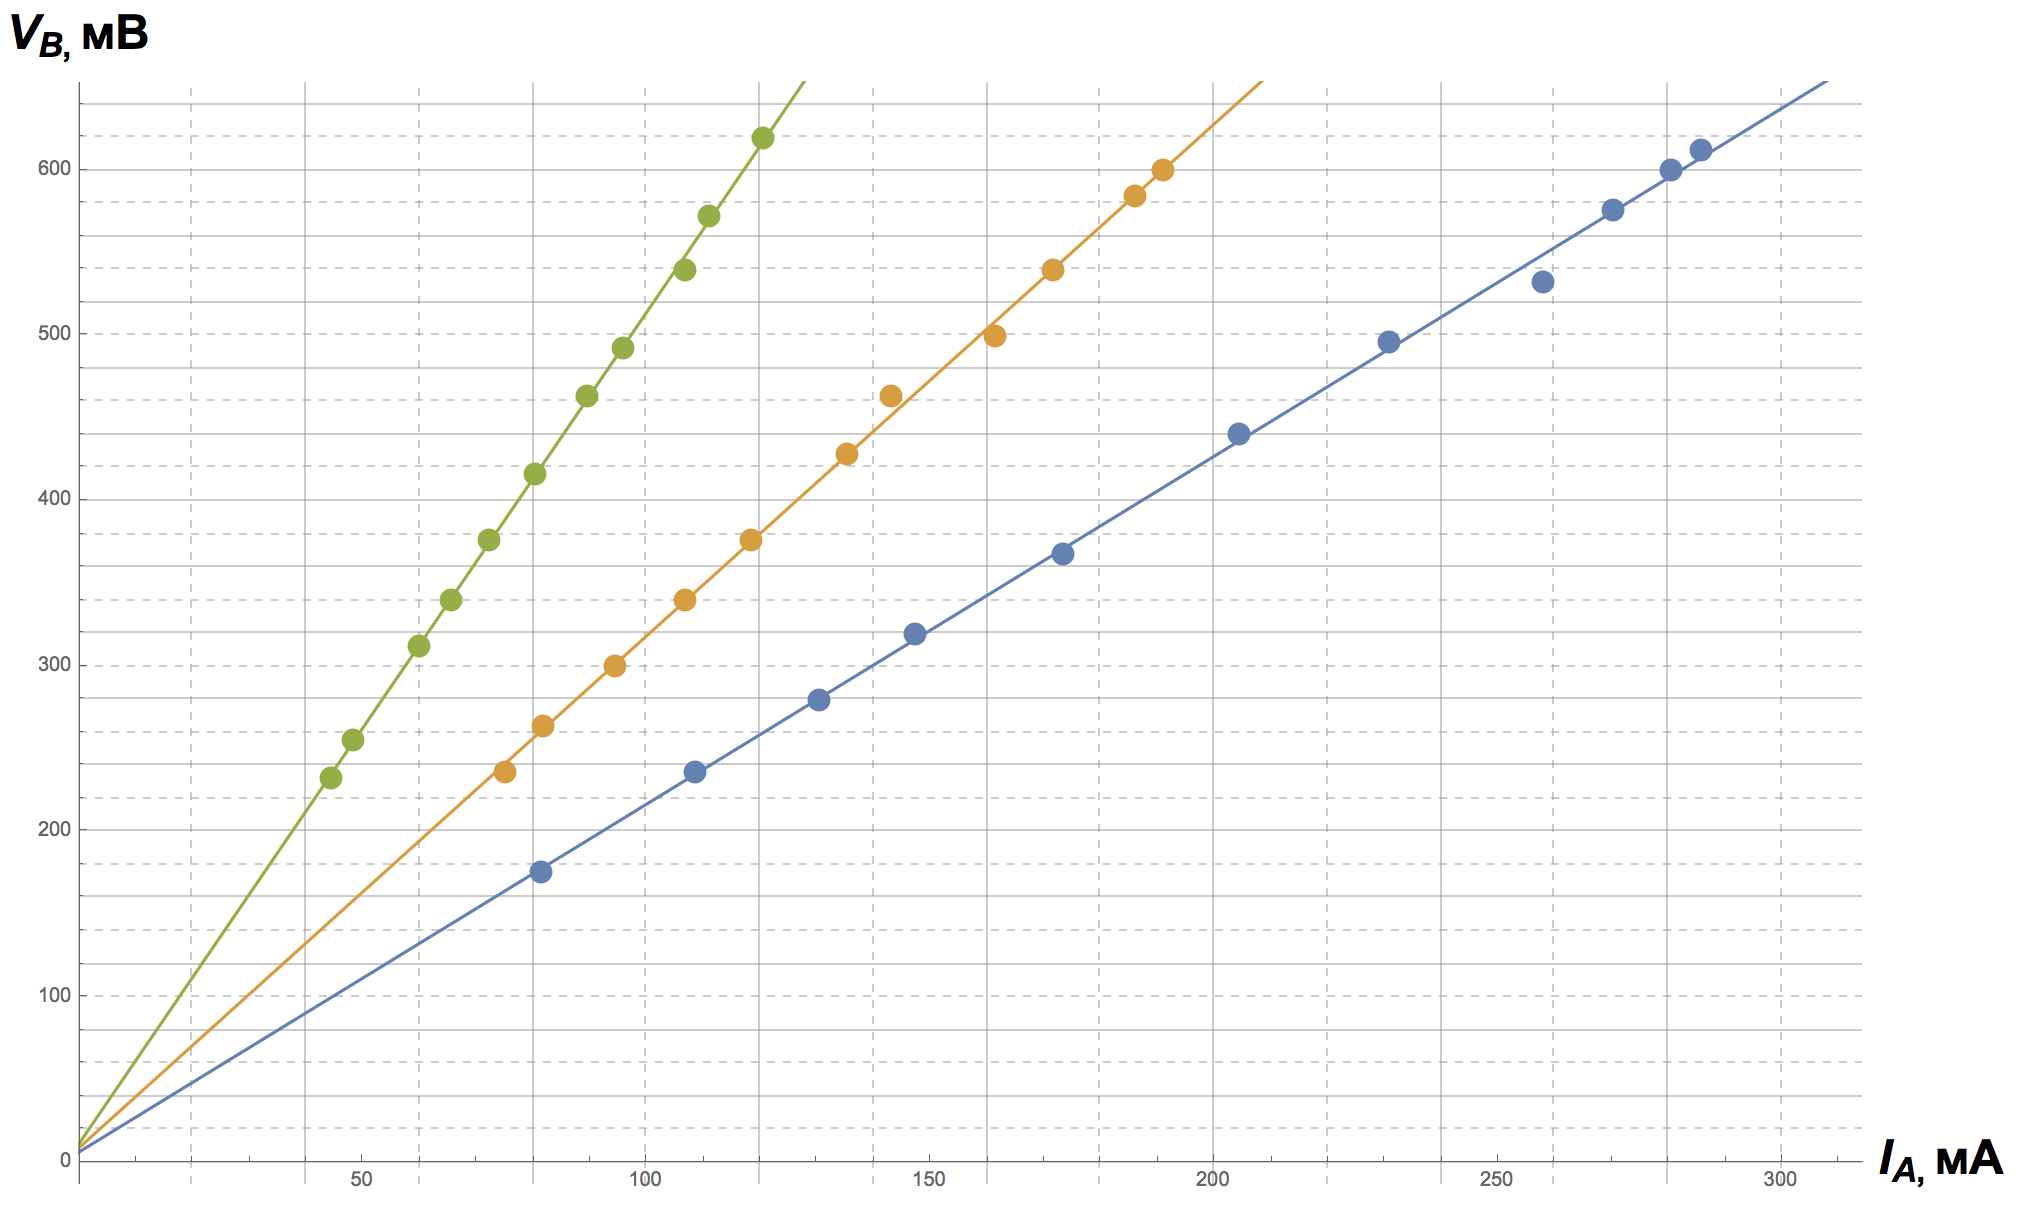
\includegraphics[width=1\textwidth]{itog}
\caption{Результаты измерений напржяения $V_B$ в зависимости от тока $I_A$ для прволок разной длины $l$ и их линейная аппроксимация $y=kx$. Отмечены инструментальные погрешности по вертикально оси ($\sigma_V=3.8\text{мВ}$). Cиния линия для $l=20\text{см}$, желтая линия для $l=30\text{см}$, зеленая линия для $l=50\text{см}$ Ввиду выбраного масштаба погрешности укладываются в размер точек.  } \label{dz1}
\end{figure}

Результаты сведены в Таблице 4. Там же для сравнения приведены результаты измерения $R$ с помощью моста постоянного тока $P4833$ с учётом его погрешности
\begin{table}[h]
\caption{Результаты измерения сопротивления проволки двумя методами}
\centering
\label{dich}
\begin{tabular}{|c|c|c|c|c|c|}
\hline
\rule{0cm}{4mm}
$l,\text{см}$ & $\overline{R}, \text{Ом}$ & $\sigma_R^\textbf{сл}, \text{Ом}$ & $\Delta_R^\text{сист}, \text{Ом}$ & $\sigma_R, \text{Ом}$ & $R_{\text{мост}}, \text{Ом}$\\ \hline
$50\pm0,1$ & 5,0274 & 0,104 & 0,0187& 0,105& $5,2284\pm0,0100$ \\ \hline
$30\pm0,1$ & 3,1564 & 0,056 & 0,0115& 0,057& $3,1781\pm 0,0100$\\ \hline
$20\pm0,1$ & 2,1438 & 0,037 & 0,0078& 0,038& $2,1568\pm0,0100$ \\ \hline
\end{tabular}
\end{table}
\newpage
\subsection{Вычисление удельного сопротивления}
По формуле ($1$) находим удельное сопротивление материала проволки, используя значение $\overline{R}$ полученные в п 4.2. Сравнивая относительные величины погрешностей величин, входящих в $(1)$, приходим к выводу, что наибольший вклад в погршеность вносит измерение диаметра проволки ($2\sigma_{d_2}/d \approx 9,9\%$), при этом вкладом ошибок остальных измерений можно пренебречь: $\sigma_\rho \approx \frac{2\sigma_{d_2}}{d}\rho$

\begin{table}[h]
\centering
\begin{tabular}{|c|c|}
\hline
$\text{№}$ опыта & $\rho, 10^{-6}\text{Ом}\cdot\text{м}$ \\ \hline
1 & 1,109$\pm0,109$\\ \hline
2 & 1,089$\pm0,108$ \\ \hline
3 & 1,041$\pm0,103$ \\ \hline
\end{tabular}
\end{table}
Усредняя результаты 3-х опытов, окончательно получим:
\[\overline{\rho}= (1,080\pm0,107)\cdot10^{-6}\text{Ом}\cdot\text{м}(\varepsilon_\rho = 9,9\%)\]
\section{Обсуждение результатов и выводы}

В работе удалось получить значение удельного сопротивления образца проволки из нихромового сплава с точностью $\sim$9,9$\%$. Табличные значения для нихрома лежат в диапозоне $\rho_{\text{табл}} = 0,97 ... 1,14\cdot10^{-6}\text{Ом}\cdot\text{м}$ в зависимости от состава. Измеренные значения $\overline{\rho}= (1,080\pm0,107)\cdot10^{-6}\text{Ом}\cdot\text{м}$ попадают в этот диапазон в пределах одного стандартного отклонения, однако погрешность результата не позволяет определить марку сплава.

Использованный в работе метод измерения сопротивлений позволил получить значения $R$ образцов с довольно высокой точностью $1,9\%$, которая ограничивалась в основном погрешностью аналогового вольтметра.

Тем не менее, точность измерения удельного сопротивления существенно ограничивается измерением диаметра проволки. Поскольку случайная ошибка измерения диаметра оказались меньше цены деления прибора (микрометра), уточнение значения диаметра за счет многократных измерений невозможно. По той же причине не удалось проверить, насколько однородной является проволка по сечению. Поэтому использование более совершенных, приборов и методов, возможно, позволило бы улучшить точность измерения диаметра, а значит и удельного сопротивления.
\end{document}
